\chapter{Vari\'aveis}
O que \'e uma vari\'avel? Na programa\c{c}\~ao uma variável consiste de um bloco de mem\'oria capaz de armazenar e representar um valor ou express\~ao e este 
pode variar durante o decorrer da execu\c{c}\~ao do programa. Em Perl uma vari\'avel pode ser declarada como apresentado na figura 2. 

\begin{figure}[!htb]
	\centering
	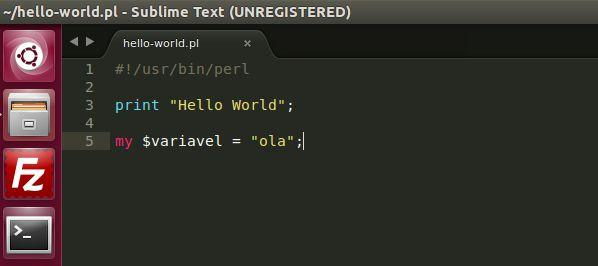
\includegraphics[width=0.5\textwidth]{../5_figuras/image2}
	\caption{Declarando-se uma vari\'avel}
\end{figure}

Toda vari\'avel possui um \$ antecedendo o seu nome, isto faz parte de sua sintaxe sendo portanto obrigat\'orio. O conte\'udo da vari\'avel \'e uma string, 
deste modo, tudo o que estiver dentro de aspas duplas ou simples \'e o conte\'udo da vari\'avel, finalizando com o ponto e v\'irgula como dito antes. Durante
a declara\c{c}\~ao da vari\'avel deve-se utilizar \textit{my} precedendo o seu nome, \textit{my \$nome\_da\_vari\'avel}.

Em Perl as vari\'aveis s\~ao dinamicamente tipadas, ou seja, n\~ao \'e necess\'ario definir o tipo de dado que aquela vari\'avel ir\'a suportar antes de 
seu uso. Segue um programa simples que realize a soma de alguns n\'umeros e escreva o seu resultado na tela.

\begin{figure}[!htb]
	\centering
	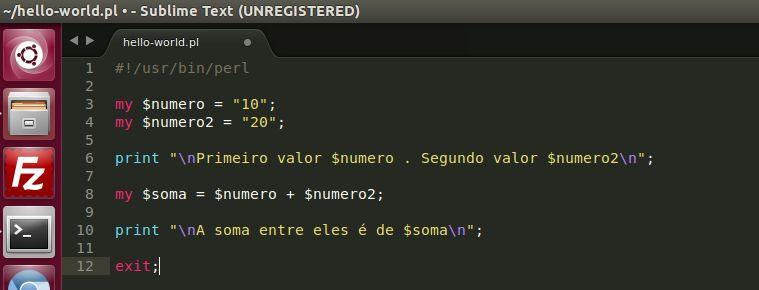
\includegraphics[width=0.5\textwidth]{../5_figuras/image3}
	\caption{Implementa\c{c}\~ao do algoritmo de soma}
\end{figure}

Na figura 3 pode-se ver que foi definido 2 vari\'aveis, \textit{\$numero = 10} e \textit{\$numero2 = 20}, logo depois \'e informado dados do usu\'ario, e 
na linha 8 \'e realizada a soma das 2 vari\'aveis que resulta no valor 30. O comando de escape ''\textit{\textbackslash n}'' indica uma quebra de linha, ele 
faz com que o conte\'udo que o procede seja escrito na pr\'oxima linha. Comandos de escape modificam a sa\'ida padr\~ao do programa. A sa\'ida do programa 
fica como apresentado na figura 4.

\begin{figure}[!htb]
	\centering
	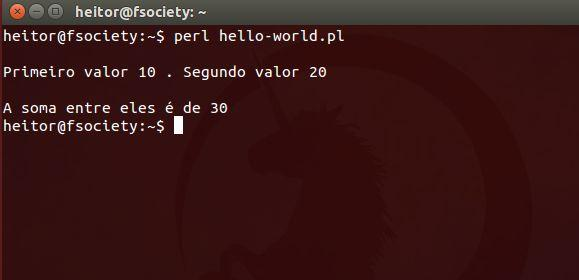
\includegraphics[width=0.4\textwidth]{../5_figuras/image4}
	\caption{Sa\'ida do algoritmo de soma}
\end{figure}

Uma lista adicional com os principais comandos de escape pode ser visto na figura 5.

\begin{figure}[!htb]
	\centering
	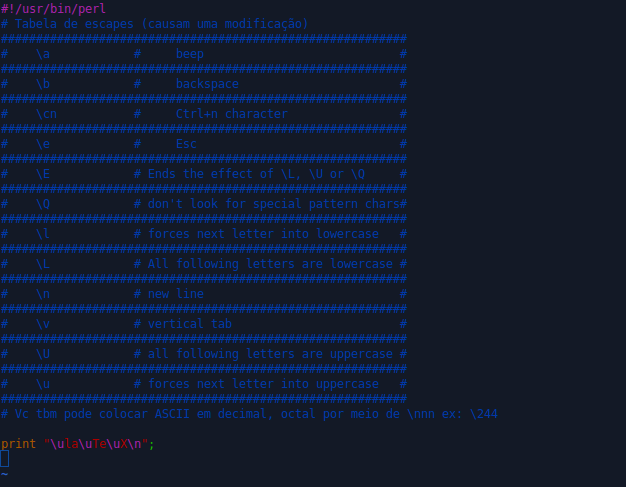
\includegraphics[width=0.45\textwidth]{../5_figuras/image5}
	\caption{Imagem 5: Trecho com principais comandos de escape}
\end{figure}

